% Author: Izaak Neutelings (Februari, 2020)
% page 8 https://archive.org/details/StaticAndDynamicElectricity
% https://tex.stackexchange.com/questions/56353/extract-x-y-coordinate-of-an-arbitrary-point-on-curve-in-tikz
% https://tex.stackexchange.com/questions/412899/tikz-calculate-and-store-the-euclidian-distance-between-two-coordinates

\documentclass[border=3pt,tikz]{standalone}
\usepackage{amsmath} % for \dfrac
\usepackage{physics}
\usepackage{tikz,pgfplots}
\usetikzlibrary{angles,quotes} % for pic (angle labels)
\usetikzlibrary{decorations.markings}
\tikzset{>=latex} % for LaTeX arrow head

\usepackage{xcolor}
\colorlet{Bcol}{violet!90}
\tikzstyle{BField}=[thick,Bcol]
\def\xmax{5.5}
\def\ymax{4}
\def\tick#1#2{\draw[thick] (#1) ++ (#2:0.03*\ymax) --++ (#2-180:0.06*\ymax)}


\begin{document}


% MAGNETIC FIELD of a CHARGED SPHERE
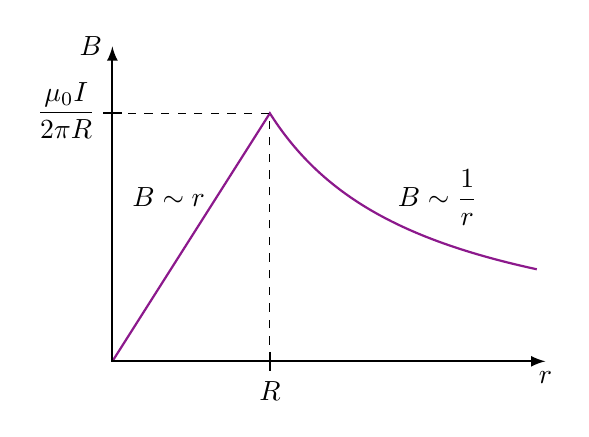
\begin{tikzpicture}
  
  \def\kQ{6.3} % mu0 / 2*pi*R
  \def\R{2.0}
  \coordinate (O) at (0,0);
  \coordinate (X) at (\xmax,0);
  \coordinate (Y) at (0,\ymax);
  \coordinate (P) at (\R,\kQ/\R);
  \coordinate (Px) at (\R,0);
  \coordinate (Py) at (0,\kQ/\R);
  
  % PLOT
  \draw[BField,samples=100,smooth,variable=\x,domain=\R:0.98*\xmax]
    (O) -- (P) -- plot(\x,\kQ/\x);
  \node[above right] at (3.5,1.6) {$B \sim \dfrac{1}{r}$};
  \node[above left] at (0.65*\R,0.46*\ymax) {$B \sim r$};
  \draw[dashed]
    (Px) -- (P) -- (Py);
  
  % AXIS
  \draw[<->,thick]
    (X) node[below] {$r$} -- (O) -- (Y) node[left] {$B$};
  \tick{Py}{ 0} node[below=-1,left=-1] {$\dfrac{\mu_0I}{2\pi R}$};
  \tick{Px}{90} node[below] {$R$};
  
\end{tikzpicture}


\end{document}
